% =====================================================================
%  1.3 Mapa
% =====================================================================
\section{Mapa das áreas de intervenção}
\label{sec:mapa}

A \autoref{fig:mapa} localiza os municípios de cada frente. A seleção está em
andamento, e o POA prevê o mapa final para dezembro de 2026. Para atualizar a
figura, basta preencher a planilha \texttt{mapa/municipios\_selecionados.csv}
(código IBGE, nome do município e frente) e executar o script
\texttt{mapa/gerar\_mapa.py}, que redesenha o arquivo \texttt{figuras/mapa-3-2-b.pdf}.

\begin{figure}[htbp]
  \centering
  \caption{Municípios de atuação do Subcomponente 3.2.b, por frente de trabalho}
  \label{fig:mapa}
  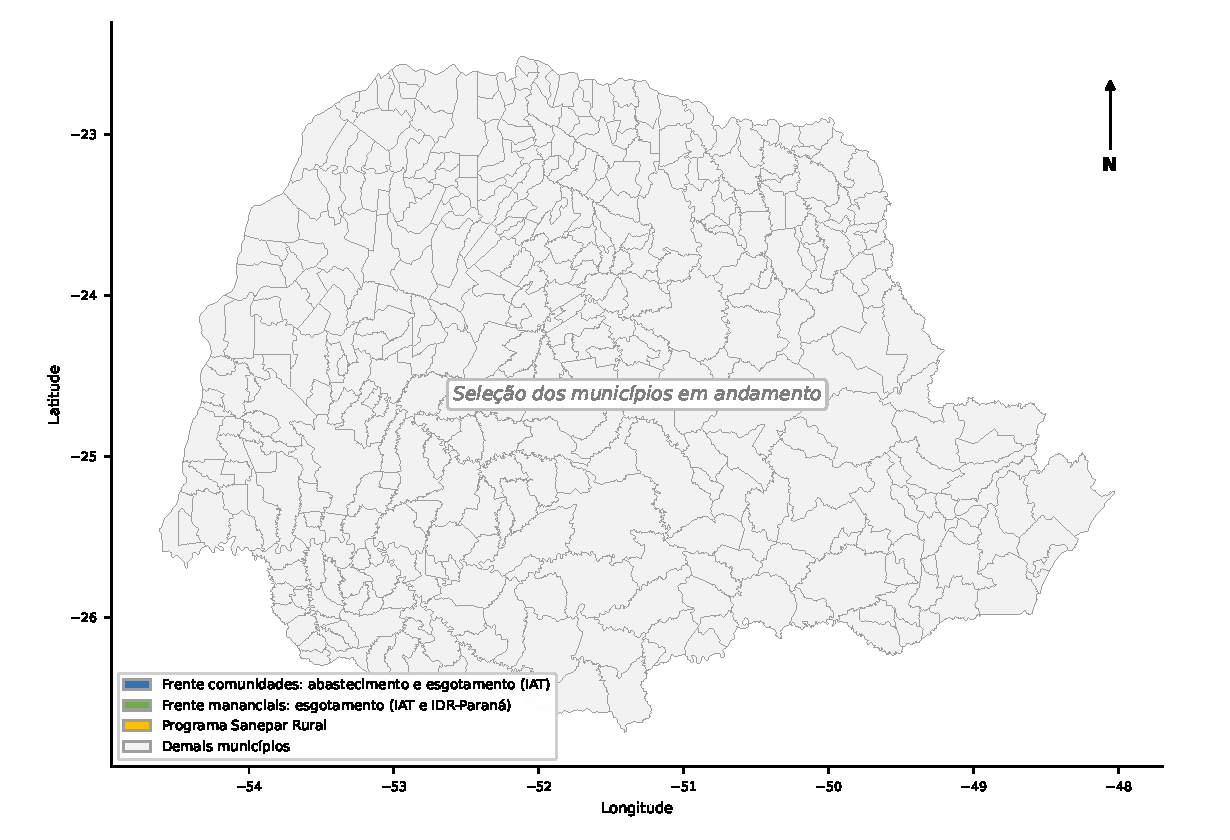
\includegraphics[width=\linewidth]{figuras/mapa-3-2-b.pdf}
  \fonte{Elaborado pelo IAT (2026) sobre a malha municipal do IBGE.}
\end{figure}

\pendencia{O Acordo de Empréstimo exige que o MOP identifique as áreas rurais
sujeitas a intervenção na Parte 3.2. Inserir o mapa com os municípios
selecionados ou descrever como a lista será aprovada com o Banco.}
